\section{Application}

\subsection{Architecture de l'application}

\paragraph{Schéma:}
L'application agit en frontal de l'api de Nexus. Les recherches se fait par Lucène (lexique.\ref{lexi:lucene}).
Sur la figure (fig.\ref{fig:schema}) on voit les flux éventuels depuis une application dans le navigateur et ceux depuis une application dans le serveur.

\begin{figure}[ht]
 \centering
 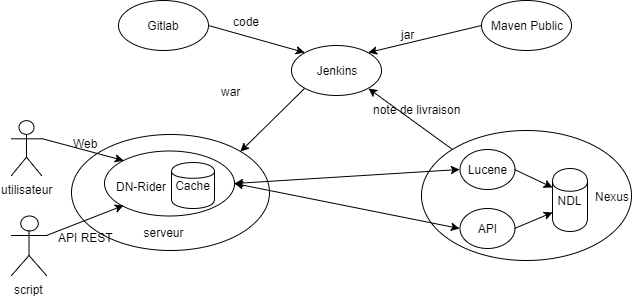
\includegraphics[width=0.7\textwidth]{schema}
 \caption{Schéma}
 \label{fig:schema}
\end{figure}

\paragraph{Modèle MVC:}
L'application suit le motif Modèle-Vue-Contrôleur.
Il est composé de trois types de modules ayant trois responsabilités différentes :
\begin{itemize}
 \item Modèle : Il n'y pas de base de données dans cette application.
       La persistance de données est assuré par Nexus et cache intégrée.
 \item Vue : La présentation de l'interface graphique.
       Elle est realisée en utilisant Bootstrap et jQuery dans cette application.
 \item Contrôleur : La logique concernant les actions effectuées par l'utilisateur.
       Réalisé en Grails dans cette application.
\end{itemize}

\paragraph{La couche service:}
On extrait les codes techniques des contrôleurs et former des services. Après, on peut les appeler depuis les contrôleurs.
Ça aide à éviter les codes répétitifs et rendre les codes métiers propre.
Par exemple, on crée un service "NexusConsumer" qui contient toutes les opérations de Nexus.
L'application pourra donc évoluer pour supporter un autre logiciel 'entrepôt' que Nexus.

\subsection{Choix des technologies}

Par principe, on choisit les technologies open-source qui conforment à l'objectif et au contexte de ce projet.

\subsubsection{Coté Serveur}

\paragraph{Grails :}
Grails est un framework open source de développement agile d'applications web basé sur le langage Groovy et sur le patron de conception Modèle-Vue-Contrôleur.
Il convient à la taille de ce projet.
De plus il y a référent compétent qui connait bien ce framework.

\paragraph{Groovy :}
Groovy est le nom d'un langage de programmation orienté objet destiné à la plate-forme Java.
Groovy utilise une syntaxe très proche de Java, par rapport à Java, il est moins verbeux et plus efficace.

\paragraph{RESTful API :}
REST (representational state transfer) est un style d'architecture pour les systèmes hypermédia distribués.
Les APIs(application programming interface) de services web qui adhèrent aux contraintes de l'architecture REST sont appelés RESTful APIs

\paragraph{Swagger :}
Swagger est une spécification pour les fichiers d'interface lisibles par machine pour décrire, la production, la consommation et la visualisation de Service Web REST.

\paragraph{Spock :}
Spock est un framework de test Java capable de gérer le cycle de vie complet d'une application logicielle.

\begin{figure}[ht]
 \centering
 
\includegraphics[width=0.6\textwidth]{technologies_back}
 \caption{Choix des Technologies : Coté Serveur}
 \label{fig:technologies_back}
\end{figure}

\subsubsection{Coté Client}

\paragraph{Bootstrap :}
Boostrap est un framework front-end qui contient une collection d'outils utiles à la création du design de sites.
C'est un ensemble qui contient des codes HTML et CSS, des formulaires, boutons, outils de navigation et autres éléments interactifs, ainsi que des extensions JavaScript en option. C'est l'un des projets les plus populaires sur la plate-forme de gestion de développement GitHub.
Cela permet de créer l'IHM d'un site facilement.

\paragraph{jQuery :}
jQuery est une bibliothèque JavaScript libre et multi-plateforme créée pour faciliter l'écriture de scripts côté client dans le code HTML des pages web.
Etant donné la complexité de l'IHM de l'application, jQuery est suffisant pour réaliser les animations et les Ajax (lexique.\ref{lexi:ajax}).

\paragraph{jQuery UI :}
jQuery UI est une collection de widgets, effets visuels et thèmes implantés avec jQuery, des feuilles de style en cascade et du HTML.

\paragraph{HTML 5, CSS 3, ECMAScript 6 :}
On essaie toujours d'utiliser les technologies récents.

\paragraph{SASS :}
Sass (Syntactically Awesome Stylesheets) est un langage de génération de feuilles de style (CSS).

\begin{figure}[ht]
 \centering
 
\includegraphics[width=0.6\textwidth]{technologies_front}
 \caption{Choix des Technologies : Coté Client}
 \label{fig:technologies_front}
\end{figure}

\subsubsection{Gestion du Code et Intégration Continue}

\paragraph{Git :}
Git est un logiciel de gestion de versions décentralisé.
Les codes sources sont géré en git et stocké sur Gitlab. L'authentification se fait par SSH.

\paragraph{Jenkins :}
Jenkins est un outil open source d'intégration continue.
Jenkins Pipeline est une suite de plug-ins qui prend en charge la mise en œuvre et l'intégration des pipelines de distribution continue dans Jenkins.
Au bout d'un mois et demi, on a la première version de l'application et on commence à faire intégration continue en utilisant Jenkins pipeline.
Chaque fois qu'il y a un commit sur la branche "master", l'application se déploie toute seule.

\begin{figure}[ht]
 \centering
 
\includegraphics[width=0.5\textwidth]{technologies_gestion}
 \caption{Choix des Technologies : Gestion du Code et Intégration Continue}
 \label{fig:technologies_gestion}
\end{figure}

\subsection{IHM}
L'interface homme-machine (IHM) de l'application est réalisé en Bootstrap, jQuery et GSP(le mécanismes de grails pour rendre les vues).
Chaque page contient une entête qui permet de naviguer entre les differentes pages.
l'entête contient des éléments suivants :
\begin{itemize}
 \item Nom de l'application, identifiant de version et de déploiement ;
 \item Quatre boutons vers les quater pages ;
 \item Un menu déroulant qui permet de basculer entre les langages (Français, Anglais, Chinois).
       Par défaut la language est configurée selon localisation.
       La fonctionnalité d'internationalization est réalisée un utilisant plugin "i18n",
       nous avons changé le format et l'encodage par défaut pour ajouter une langage non-latino.
\end{itemize}

L'application contient principalement les cinq écrans suivants :
\begin{itemize}
 \item Page d'accueil ;
 \item Page recherche ;
 \item Page comparison ;
 \item Page validation ;
 \item Page edition.
\end{itemize}

%page d'accueil
\subsubsection{Paged'accueil (fig.\ref{fig:page_home})}
Cette page contient des élements suivants :
\begin{itemize}
 \item Un champ de recherche qui ramène à la page recherche ;
 \item Une fenêtre modale (fig.\ref{fig:modal_setting}) pour la configuration personnalisée ;
 \item Des boutons comme accès rapide vers la page recherche ;
 \item Un pied de page qui renvoie vers la documentation, les codes sources de l'application et la documentation de l'api REST.
\end{itemize}

\begin{figure}[ht]
 \centering
 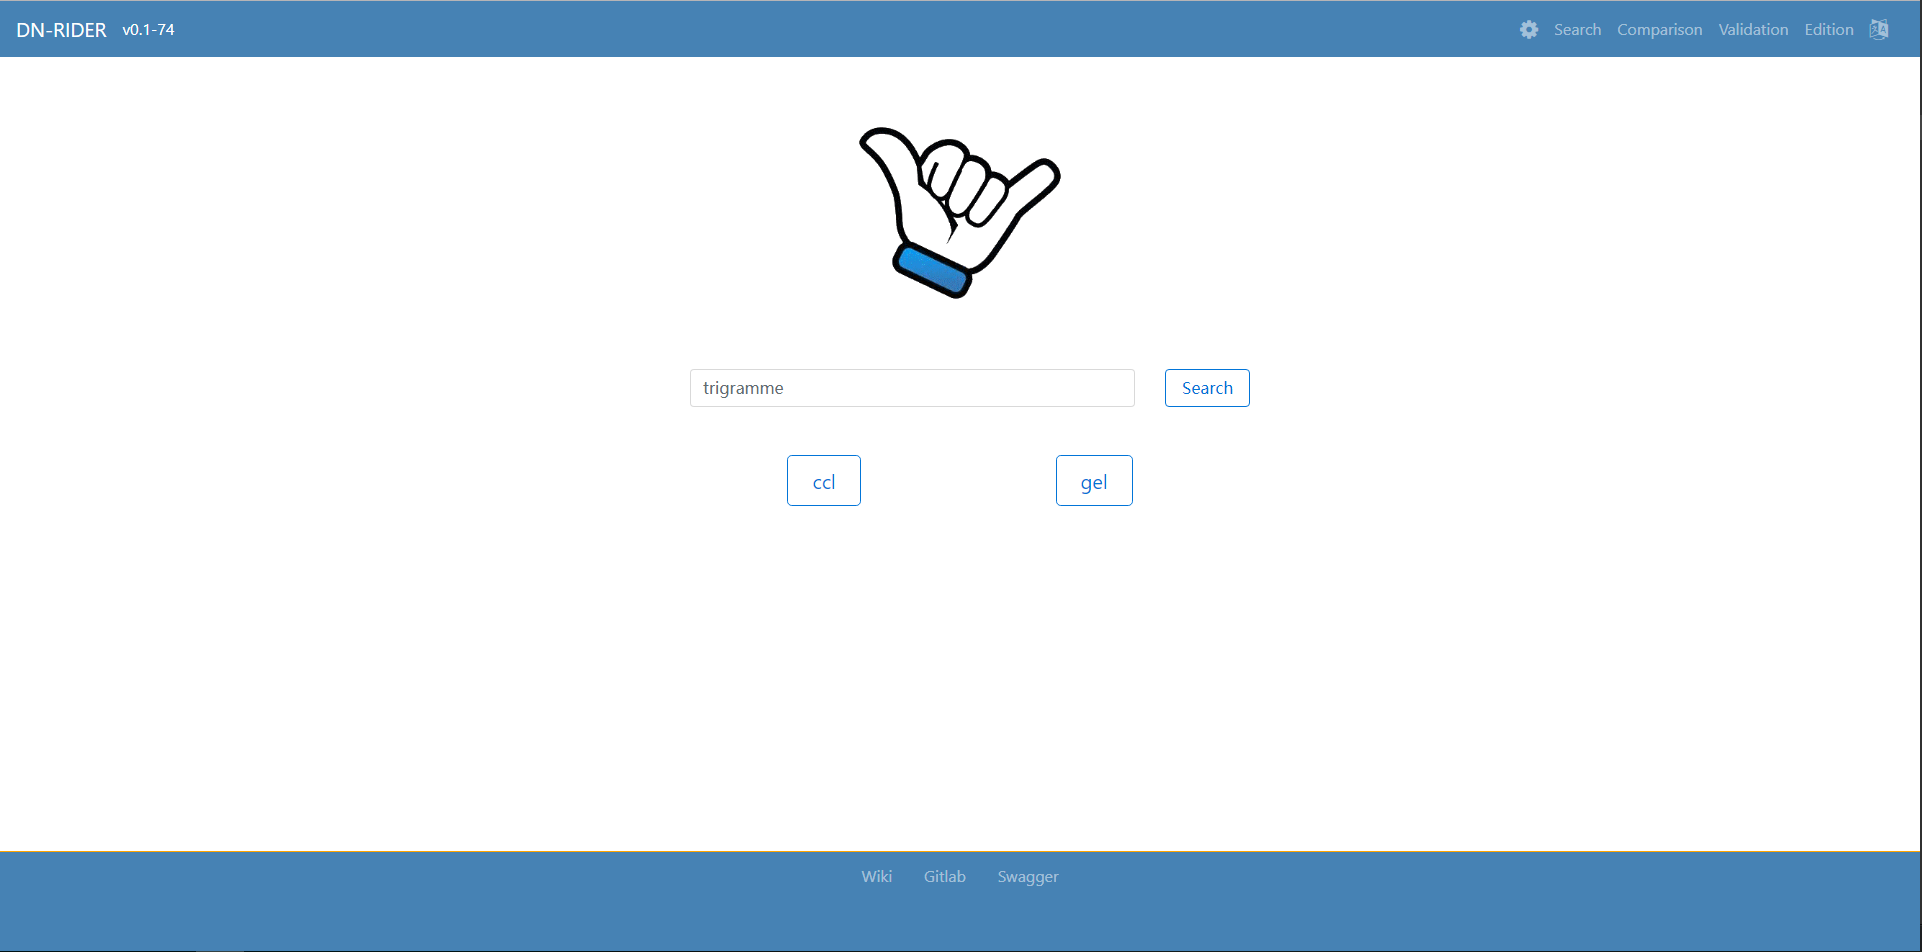
\includegraphics[width=0.8\textwidth]{page_home}
 \caption{La page d'accueil}
 \label{fig:page_home}
\end{figure}

\begin{figure}[ht]
 \centering
 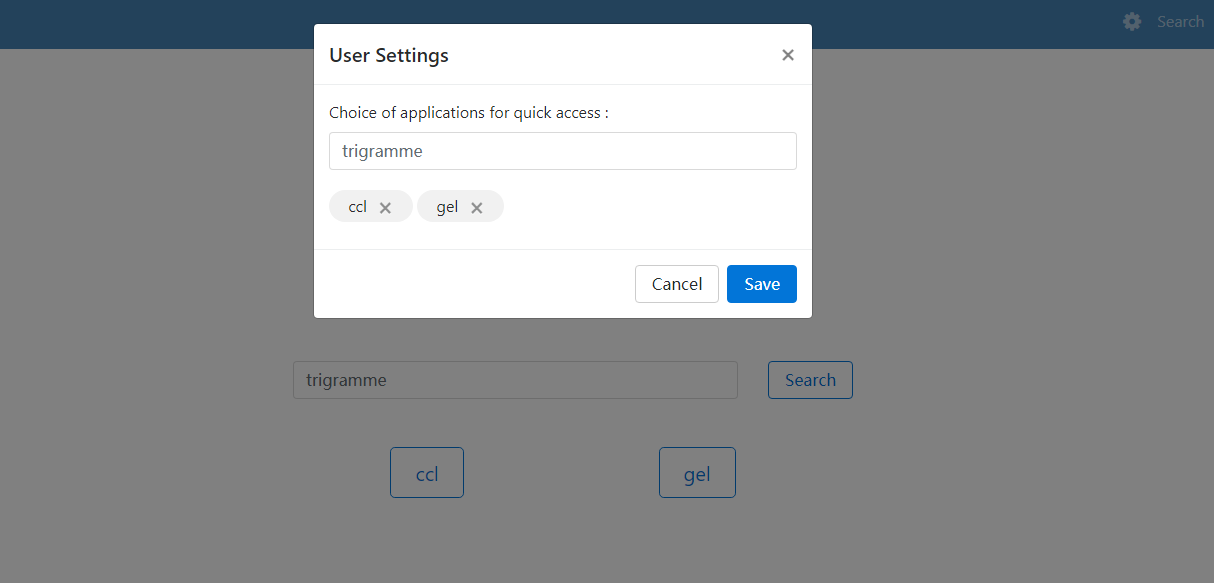
\includegraphics[width=0.6\textwidth]{modal_setting}
 \caption{Le modal configuration}
 \label{fig:modal_setting}
\end{figure}

%page recherche
\subsubsection{Page recherche (fig.\ref{fig:page_search})}
Cette page permet de choisir une note de livraison et l'afficher.

Elle contient des éléments suivants :
\begin{itemize}
 \item Un sidebar collapsible qui contient un formulaire pour choisir les notes de livraisons.
       On peut filter par le type de release et la grammaire de l'expression régulière (regex) ;
 \item Une note de livraison affichée au format json manipulative.
       L'affichage de json est réalisé avec un plugin jQuery ;
 \item Des boutons qui permettent de swicher le format d'affichage et des liens vers la page validation et l'application Nexus.
\end{itemize}

\begin{figure}[ht]
 \centering
 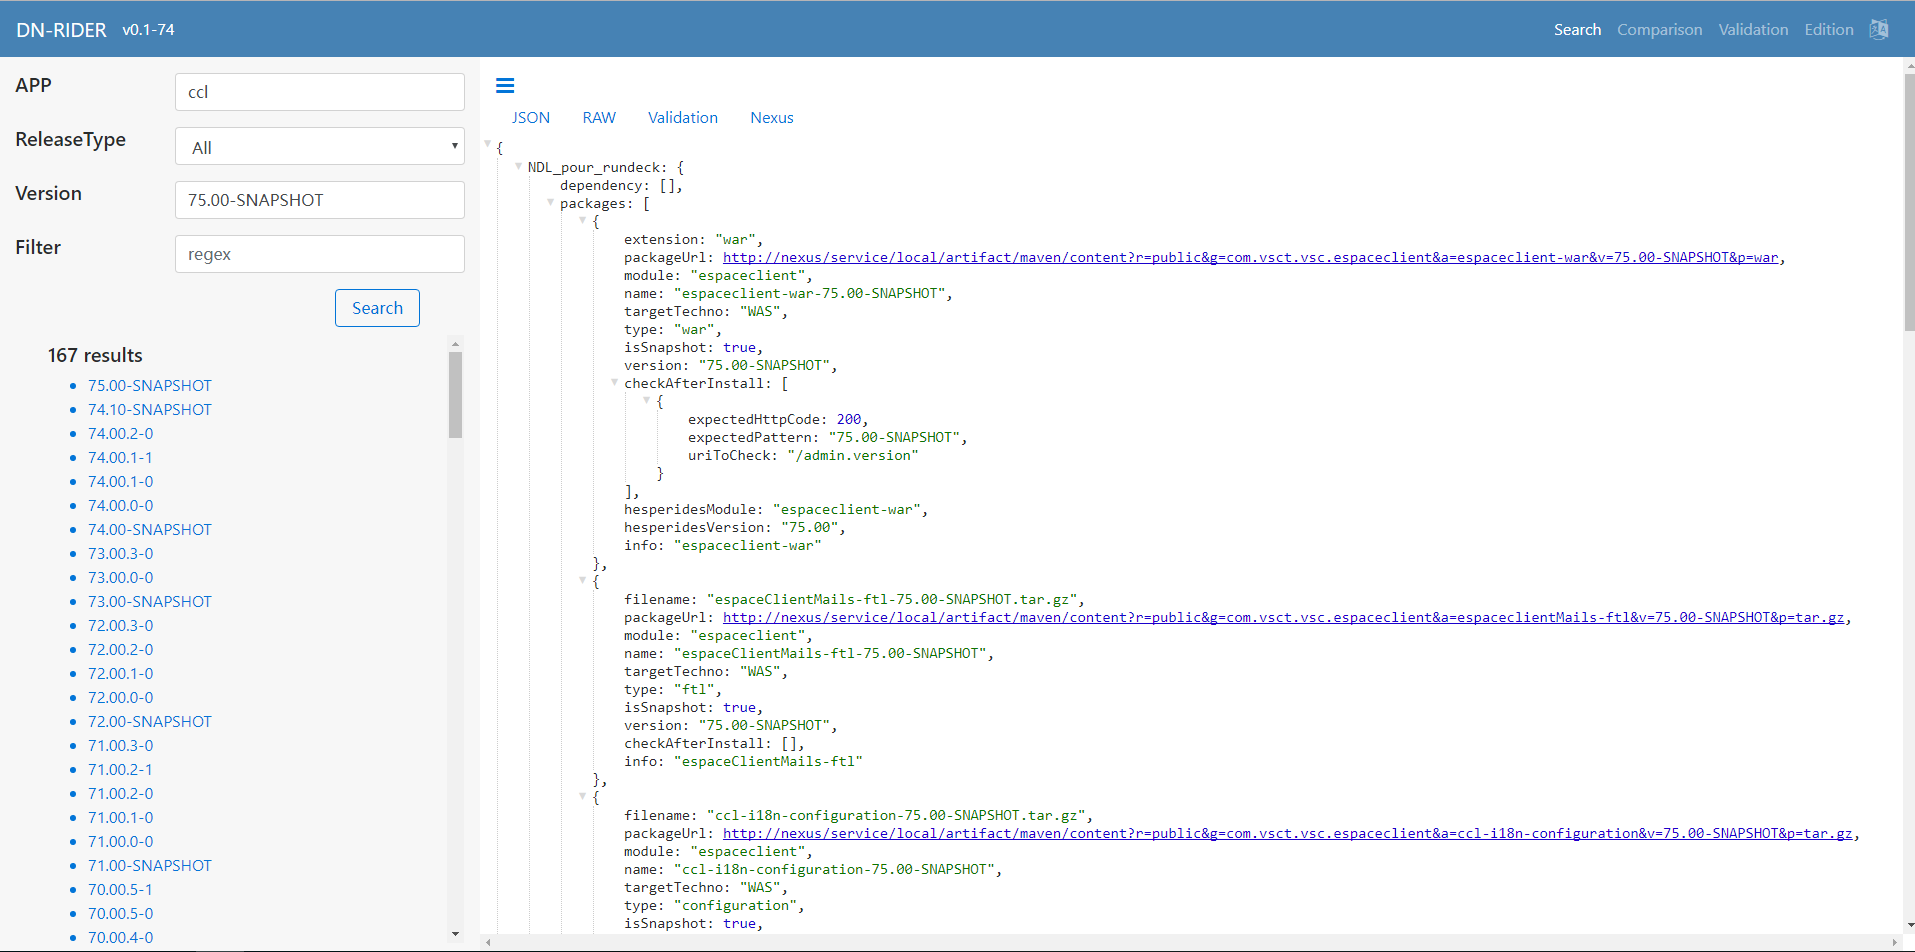
\includegraphics[width=0.8\textwidth]{page_search}
 \caption{La page recherche}
 \label{fig:page_search}
\end{figure}

%page comparaison
\subsubsection{Page comparaison (fig.\ref{fig:page_comparaison})}
Cette page permet de comparer les différentes versions de notes de livraisons d'une trigramme (lexique.\ref{lexi:trigramme}).

Elle contient des éléments suivants :
\begin{itemize}
 \item Un sidebar collapsible qui contient un formulaire pour choisir les notes de livraisons ;
 \item Un tableau qui compare les packages des notes de livraisons, le contenu des packages se présentent dans un popover sous format json manipulatif.
\end{itemize}

\begin{figure}[ht]
 \centering
 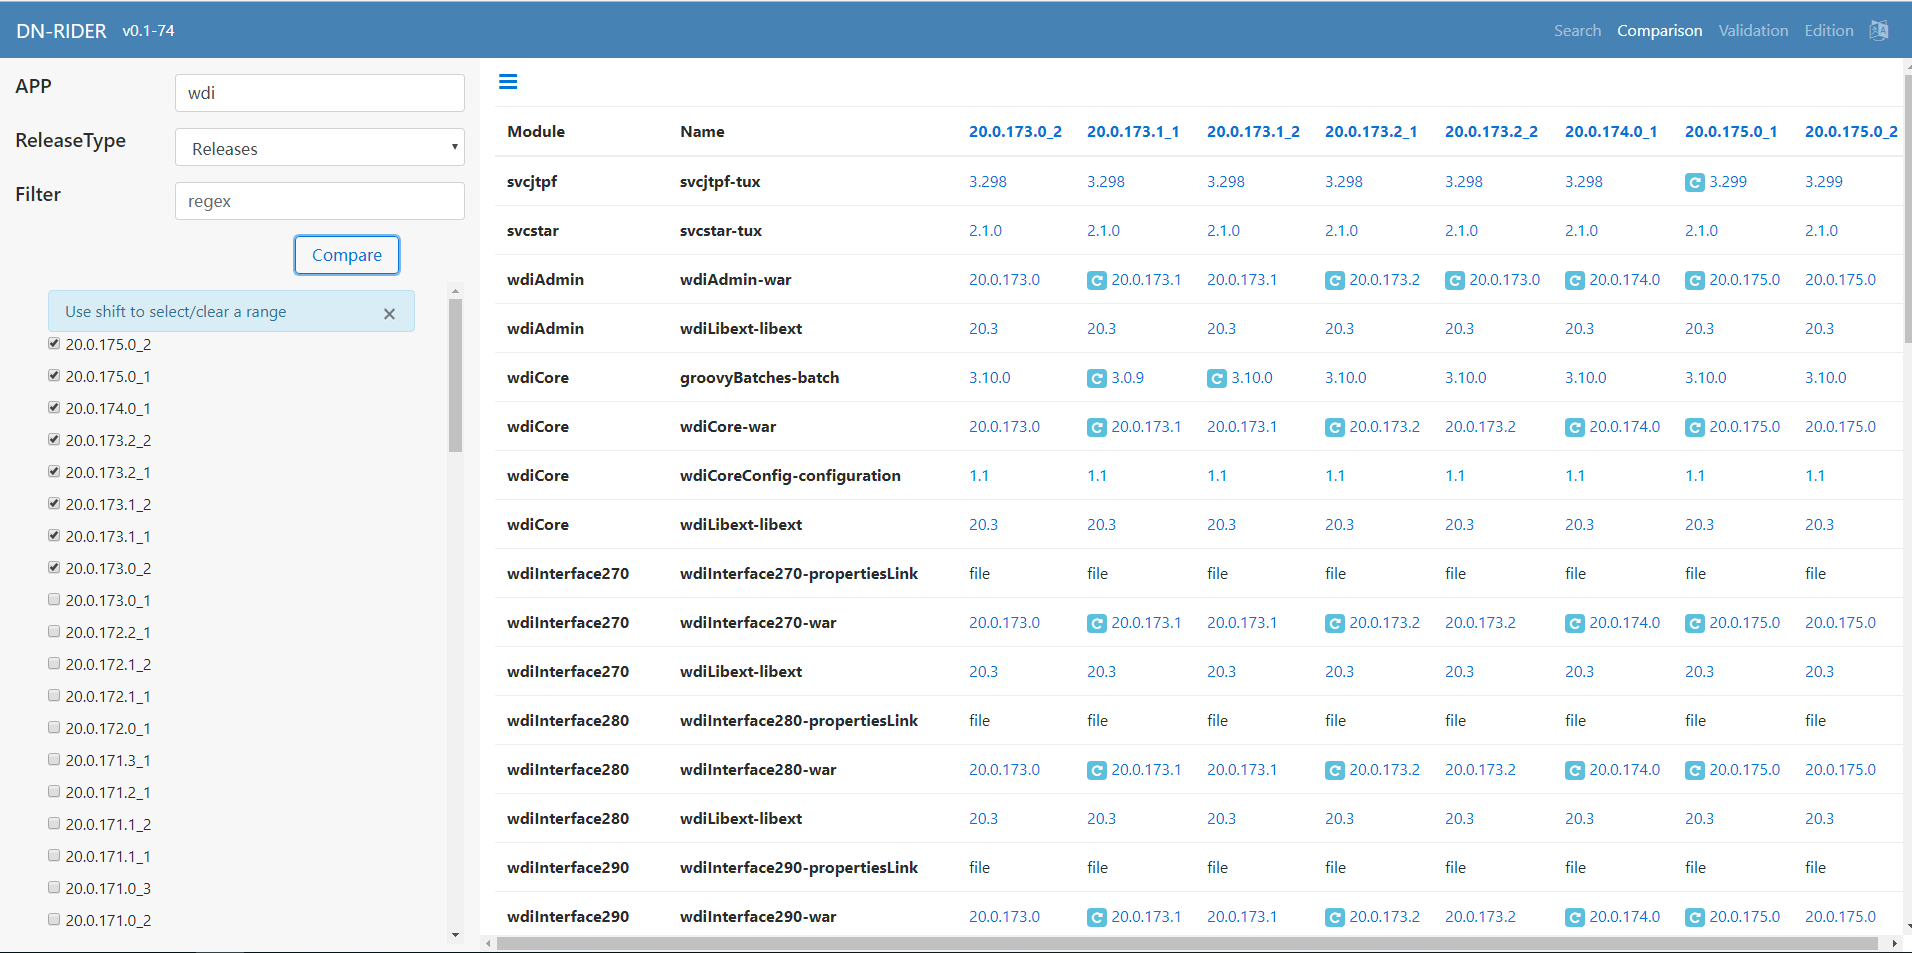
\includegraphics[width=0.8\textwidth]{page_comparison}
 \caption{La page comparaison}
 \label{fig:page_comparaison}
\end{figure}

%page validation
\subsubsection{Page validation (fig.\ref{fig:page_validation})}
Cette page permet de vérifier si une note de livraison est validée selon un json schéma.

Elle contient des éléments suivants :
\begin{itemize}
 \item Une zone qui permet d'éditer une note de livraison ;
 \item Un bouton qui ramène vers une page qui affiche le schéma ;
 \item Une fenêtre qui affiche les résultats de validation. Il y a trois types de résultats possibles :
       \begin{itemize}
        \item Json non valide :
              Afficher la position de l'erreur et un lien vers l'erreur dans la zone d'édition ;
        \item Schéma non valide :
              Afficher les informations erreurs détaillées au format json ;
        \item Valide :
              Message de réussite.
       \end{itemize}
\end{itemize}

\begin{figure}[ht]
 \centering
 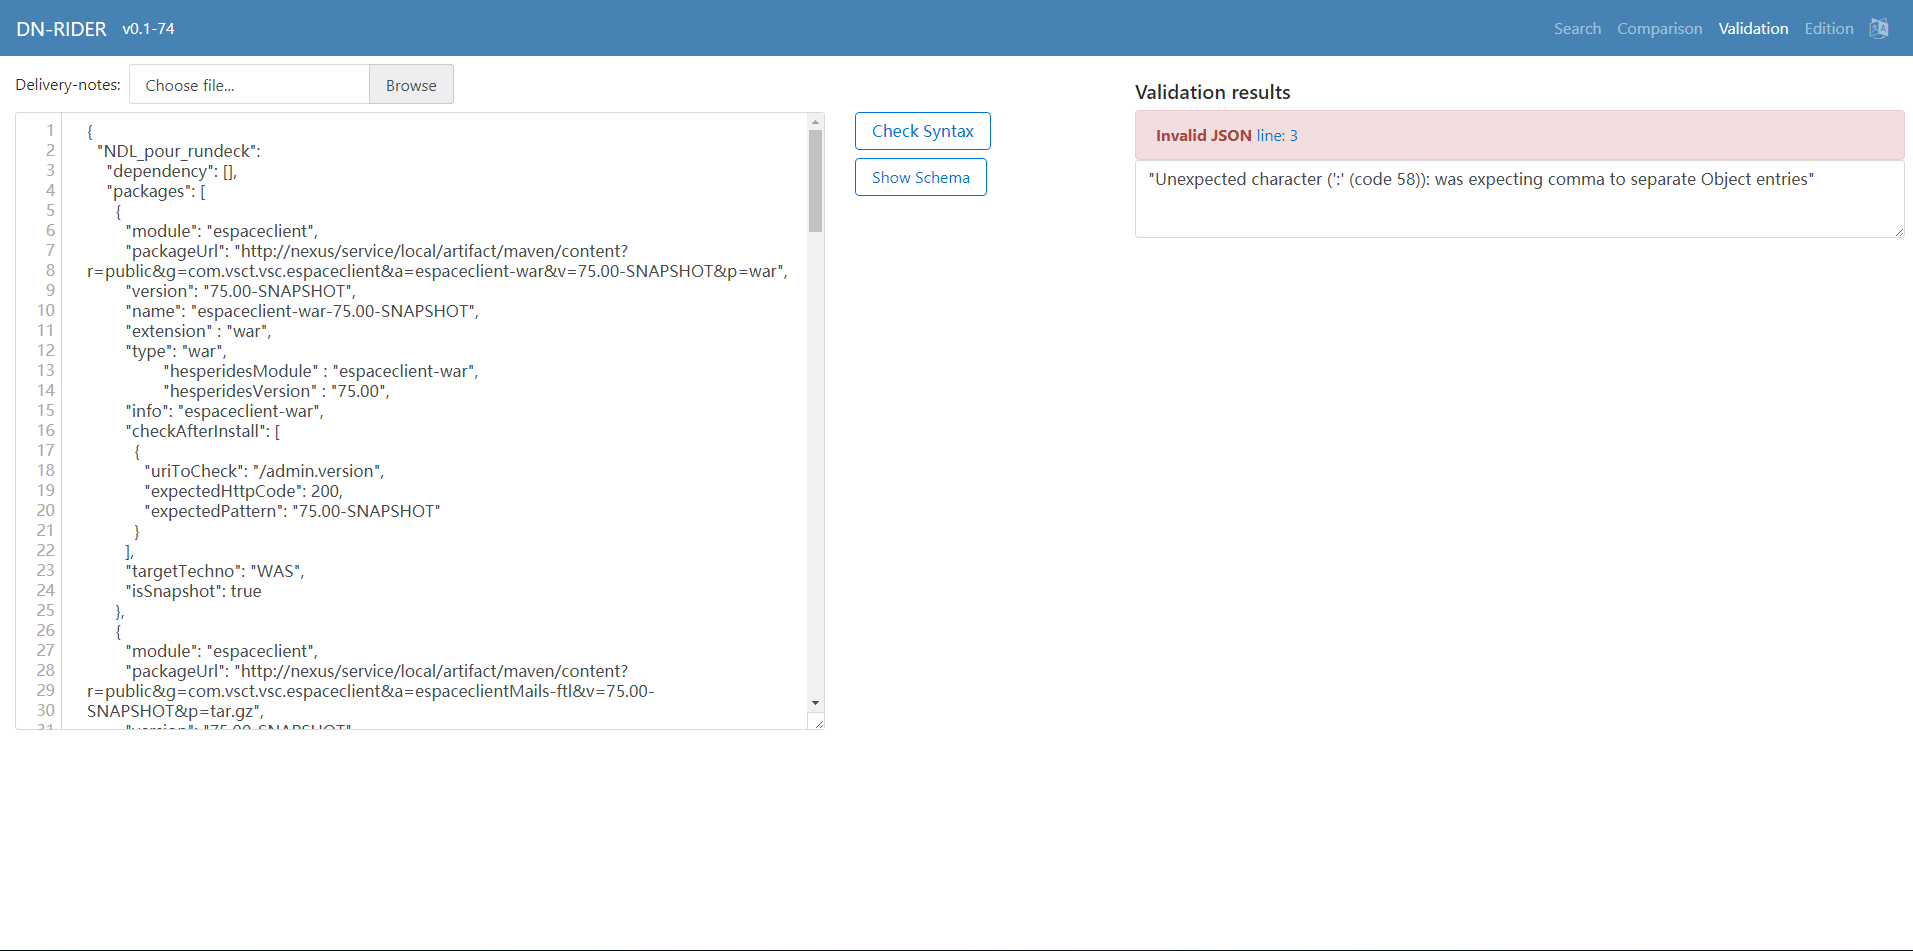
\includegraphics[width=0.8\textwidth]{page_validation}
 \caption{La page validation}
 \label{fig:page_validation}
\end{figure}

%page edition
\subsubsection{Page edition (fig.\ref{fig:page_edition})}
Cette page permet d'éditer, valider et stocker une note de livraison.

Elle contient des éléments suivants :
\begin{itemize}
 \item Un sidebar collapsible qui contient un formulaire pour choisir les notes de livraisons ;
 \item Une zone qui permet d'éditer une note de livraison ;
 \item Une fenêtre qui affiche les résultats de validation ;
 \item Un modal (fig.\ref{fig:modal_save}) qui permet de stocker la note de livraison.
\end{itemize}

\begin{figure}[ht]
 \centering
 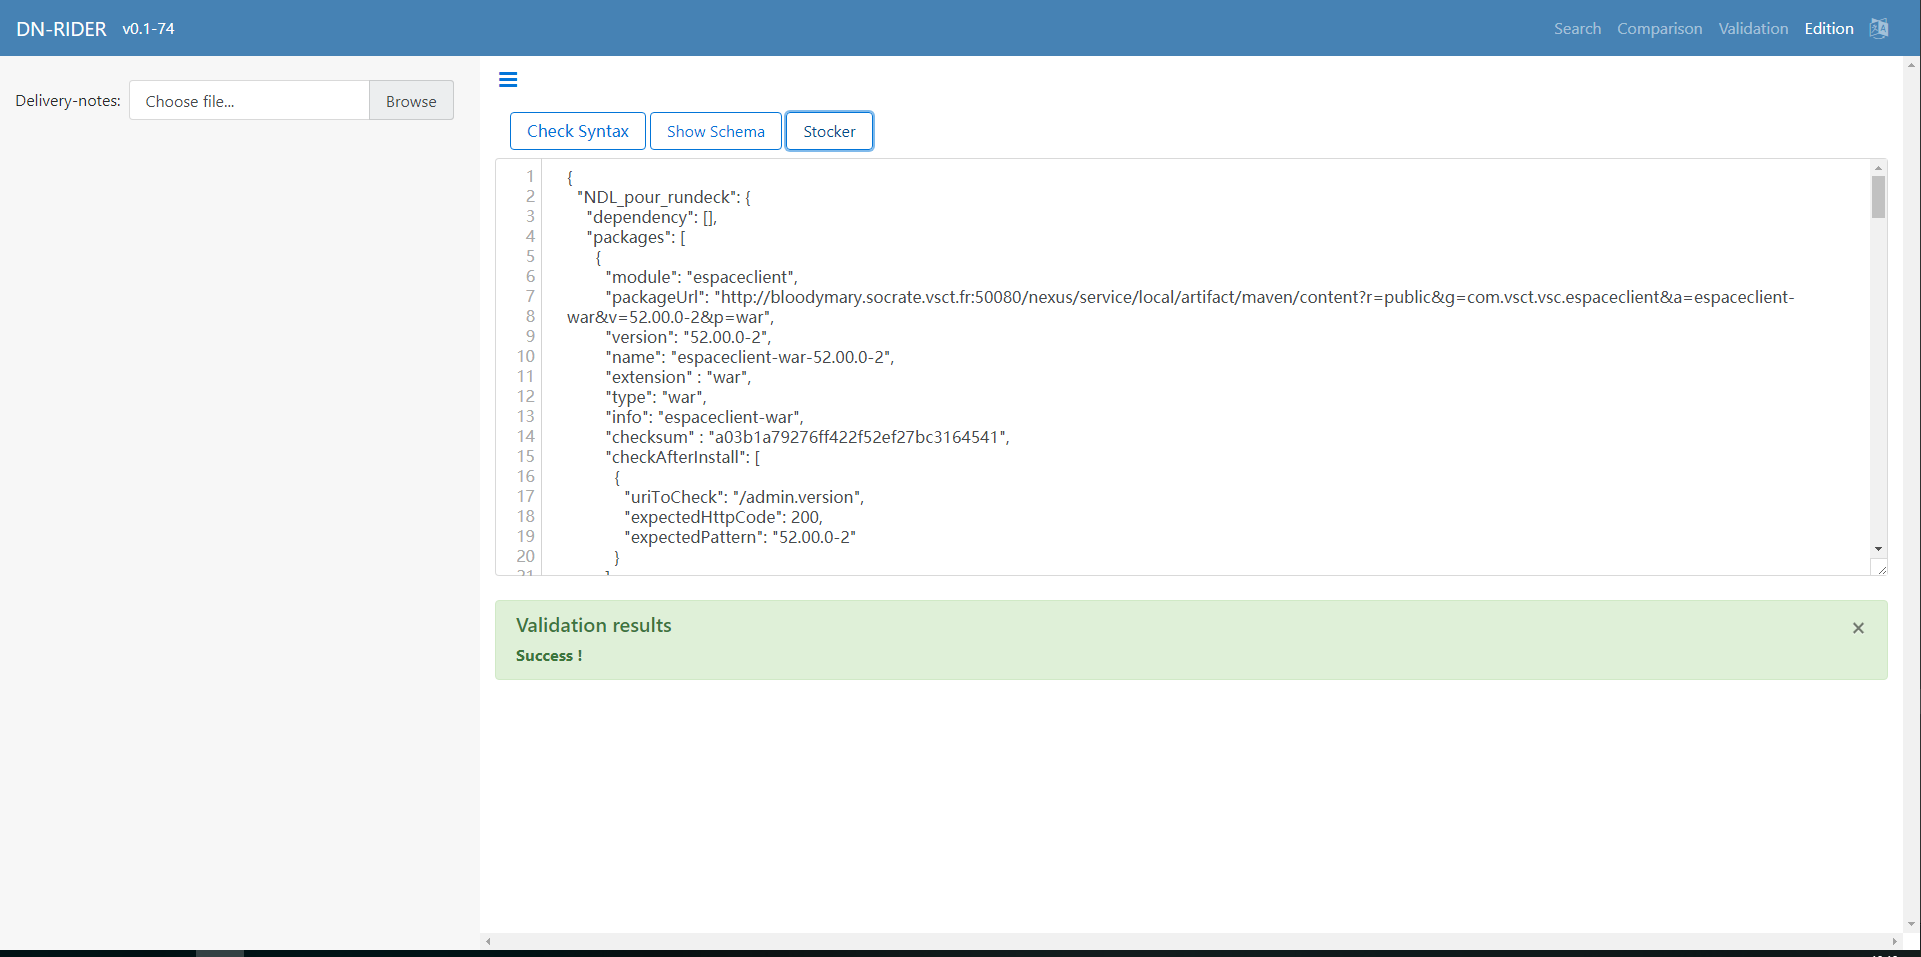
\includegraphics[width=0.8\textwidth]{page_edition}
 \caption{La page edition}
 \label{fig:page_edition}
\end{figure}

\begin{figure}[ht]
 \centering
 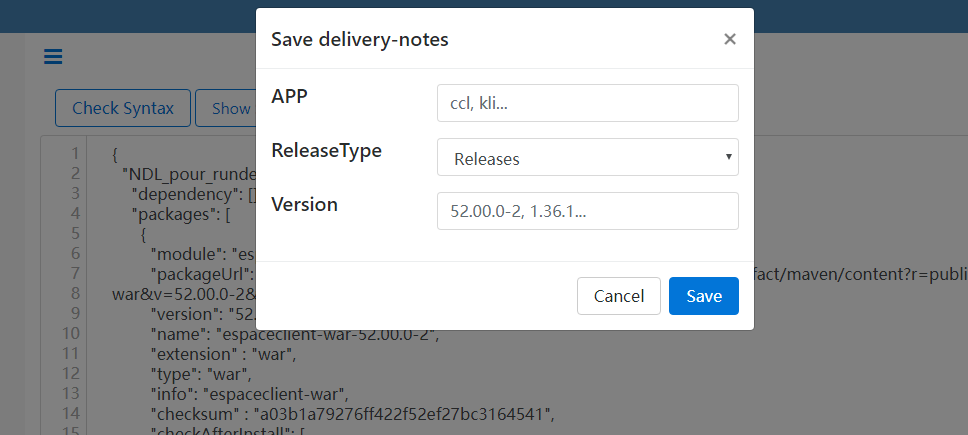
\includegraphics[width=0.6\textwidth]{modal_save}
 \caption{Le modal configuration}
 \label{fig:modal_save}
\end{figure}

\subsection{Api REST}
L'application fournie une interface api REST.
Comme dans l'IHM , l'api permet de chercher, valider, stocker des notes de livraison.
En plus, elle permet de supprimer des notes de livraison.
Ce qui est différent de l'IHM, on ne peut pas comparer les différents versions d'une trigramme, mais on peut obtenir le contenu d'un package d'une note de livraison.

L'application fournie aussi une interface graphique (fig.\ref{fig:page_swagger}) réalisé en Swagger pour la documentation de l'api.
Il est réalisé en utilisant un plugin et en ajoutant des annotations dans les contrôleurs.

\begin{figure}[ht]
 \centering
 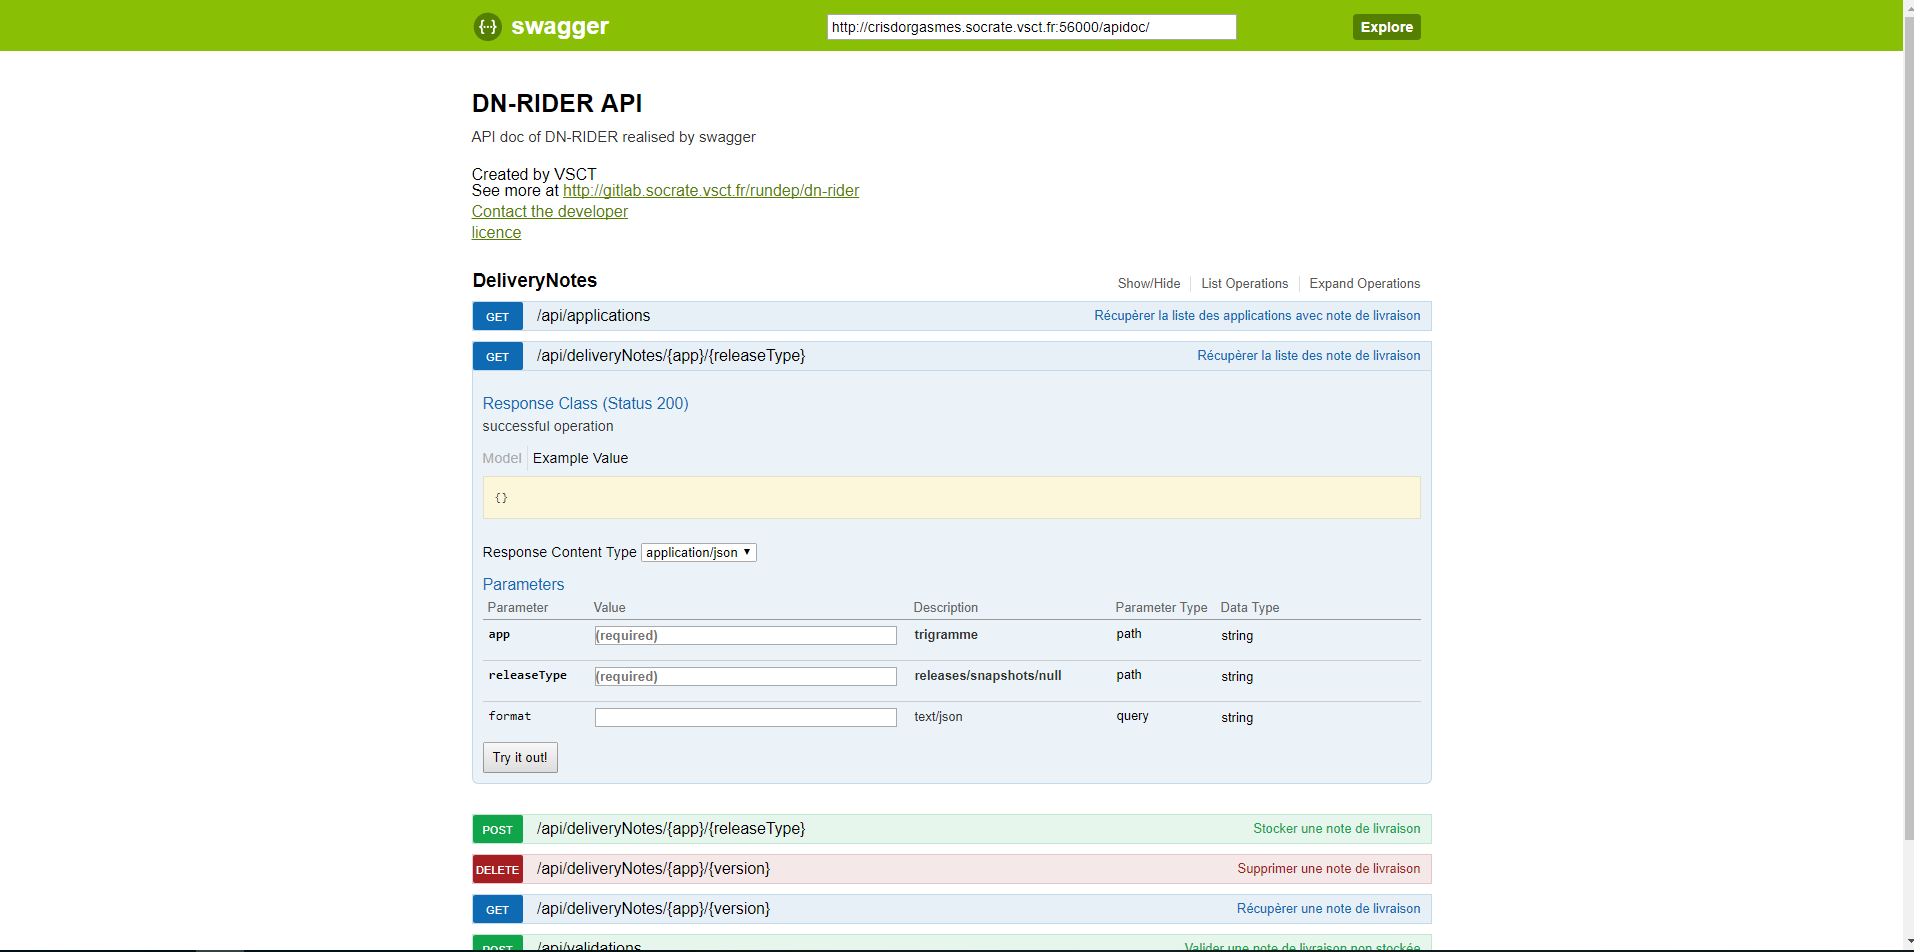
\includegraphics[width=0.8\textwidth]{page_swagger}
 \caption{La page swagger}
 \label{fig:page_swagger}
\end{figure}

\subsection{Intégration Continue}
Afin d'améliorer la qualité du code et du produit final et faciliter le déploiement de l'application, on pratique les principes de l'intégratioin continue.
L'intégration continus de l'application se réalise en utilisant git et jenkins pipeline.

Les codes sources sont gérés en git et stocké dans Gitlab.
Au début on a défini des actions à réaliser obligatoirement avant de faire "git push" :
\begin{itemize}
 \item Faire relire le code par un tiers ;
 \item Faire valider par un tiers que la feature développée fonctionne comme attendu ;
 \item Valider la nouvelle fonction par un ou des tests ;
 \item Exécuter grails command "test-app".
\end{itemize}

Le pipeline (fig.\ref{fig:jenkins}) contient les étapes suivantes:
\begin{itemize}
 \item "checkout" : Récupérer les codes de Gitlab;
 \item "versioning" : Modifier la version de l'application selon le numéro de déploiement sur Jenkins;
 \item "build" : Builder l'applcation;
 \item "deploy" : Copier le war excutable sur le serveur de production;
 \item "run" : Exécuter l'application.
\end{itemize}

\begin{figure}[ht]
 \centering
 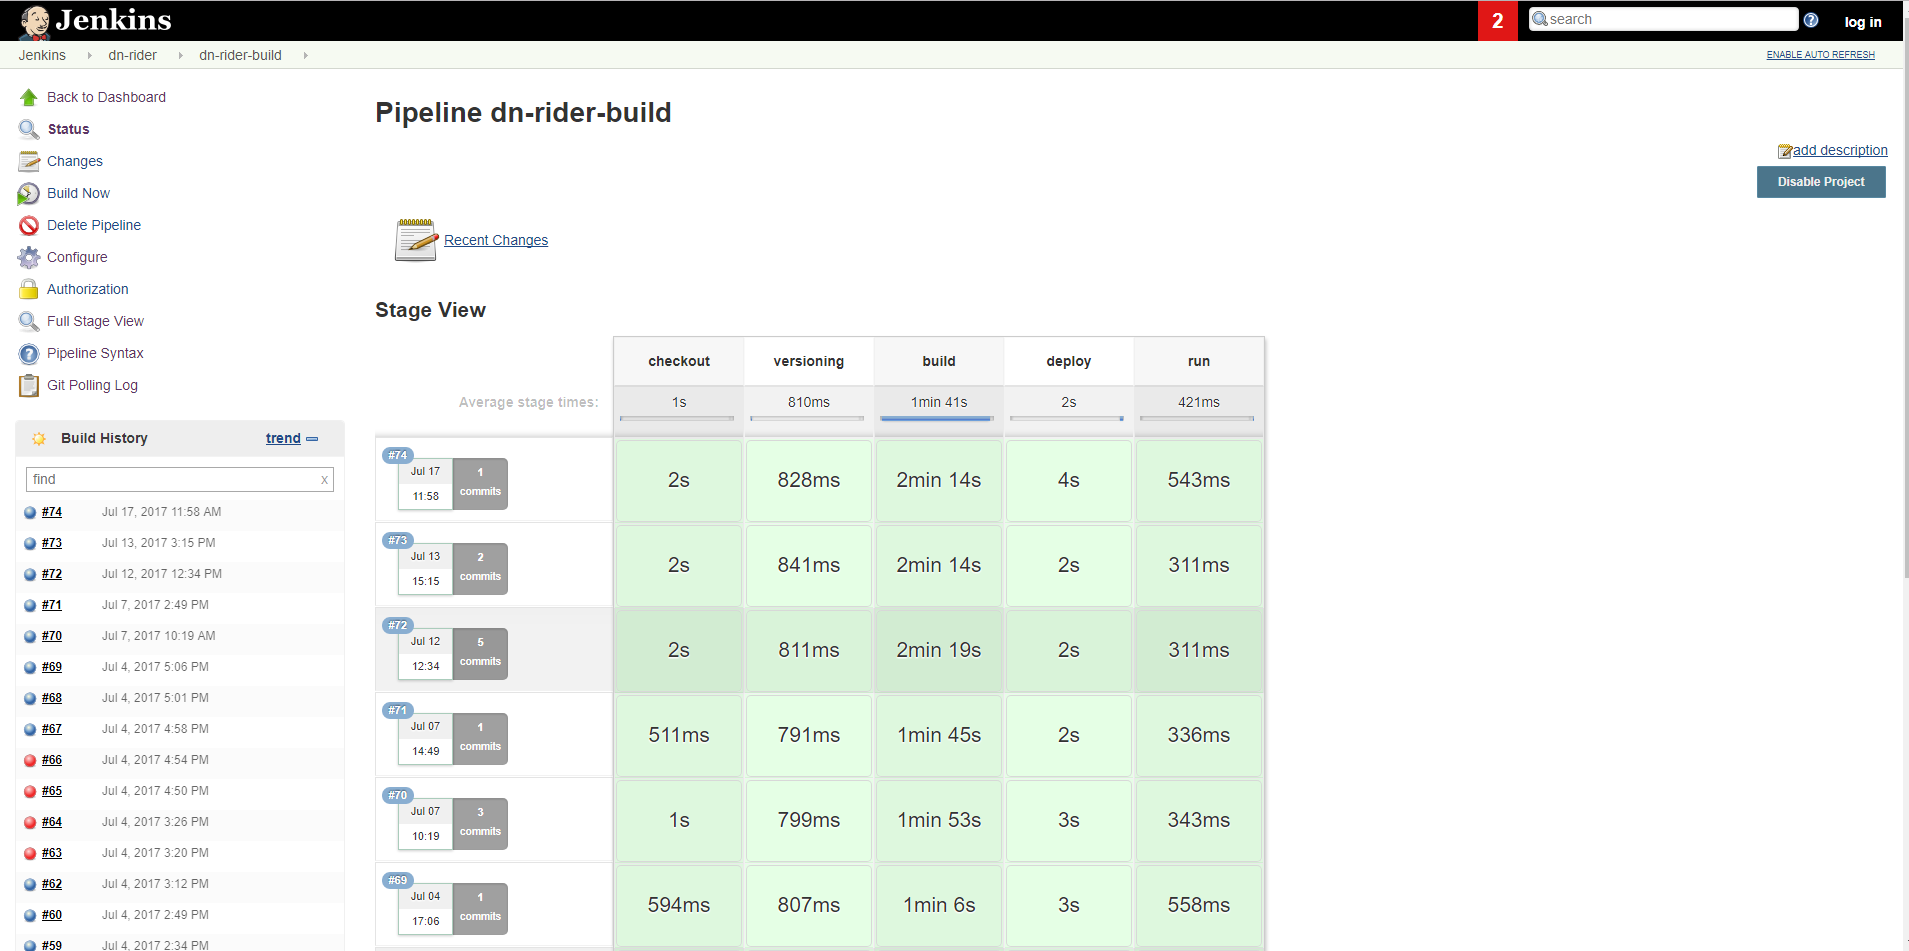
\includegraphics[width=0.8\textwidth]{jenkins}
 \caption{Jenkins}
 \label{fig:jenkins}
\end{figure}

\subsection{Test}

Les tests sont faits pour assurer le bon fonctionnement.
Ils sont à lancer avant chaque confirmation de modification de code et chaque déploiement. (fig.\ref{fig:test})

\begin{figure}[ht]
 \centering
 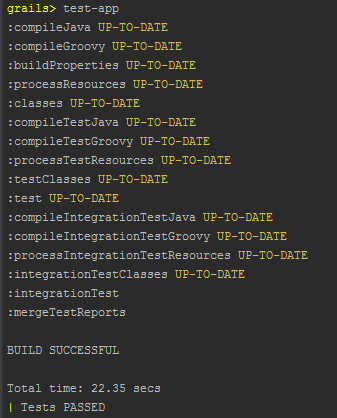
\includegraphics[width=0.4\textwidth]{test}
 \caption{Test}
 \label{fig:test}
\end{figure}

Les tests contientent des parties suivantes :
\begin{itemize}
 \item les tests d'intégration:
       Dans le test d’intégration, chacun des modules indépendants du logiciel est assemblé et testé dans l’ensemble.
       Ils sont réalisés en utilisant le framework "Spock" et ils ont couvert l'ensemble des fonctionnalités de l'api REST.
 \item les tests fonctionnels:
       Les tests fonctionnels sont pour objectif de  vérifier que les fonctionnalités demandées sont bien supportées.
       Ils sont prévu pour la partie IHM.
\end{itemize}

L'automatisation de test sur Jenkins est prévu.

\clearpage
